\documentclass[12pt, a4paper, oneside]{article}
\usepackage{astronotes}

\begin{document}

\pagestyle{fancy}
\fancyhf{}
\lhead{\textbf{กิตติพัศ พงศ์อรุโณทัย}\\{\today}}
\rhead{\textbf{ReadMe\_02}\\ปฐมบทสู่ดาราศาสตร์}
\cfoot{\thepage}

\begin{titlepage}
    \centering
    
    %
\includegraphics[width=0.15\textwidth]{img/sklogo.png}
    %
\includegraphics[width=0.15\textwidth]{img/kvislogo.png}
    %
\includegraphics[width=0.15\textwidth]{img/mwitlogo.png}
    %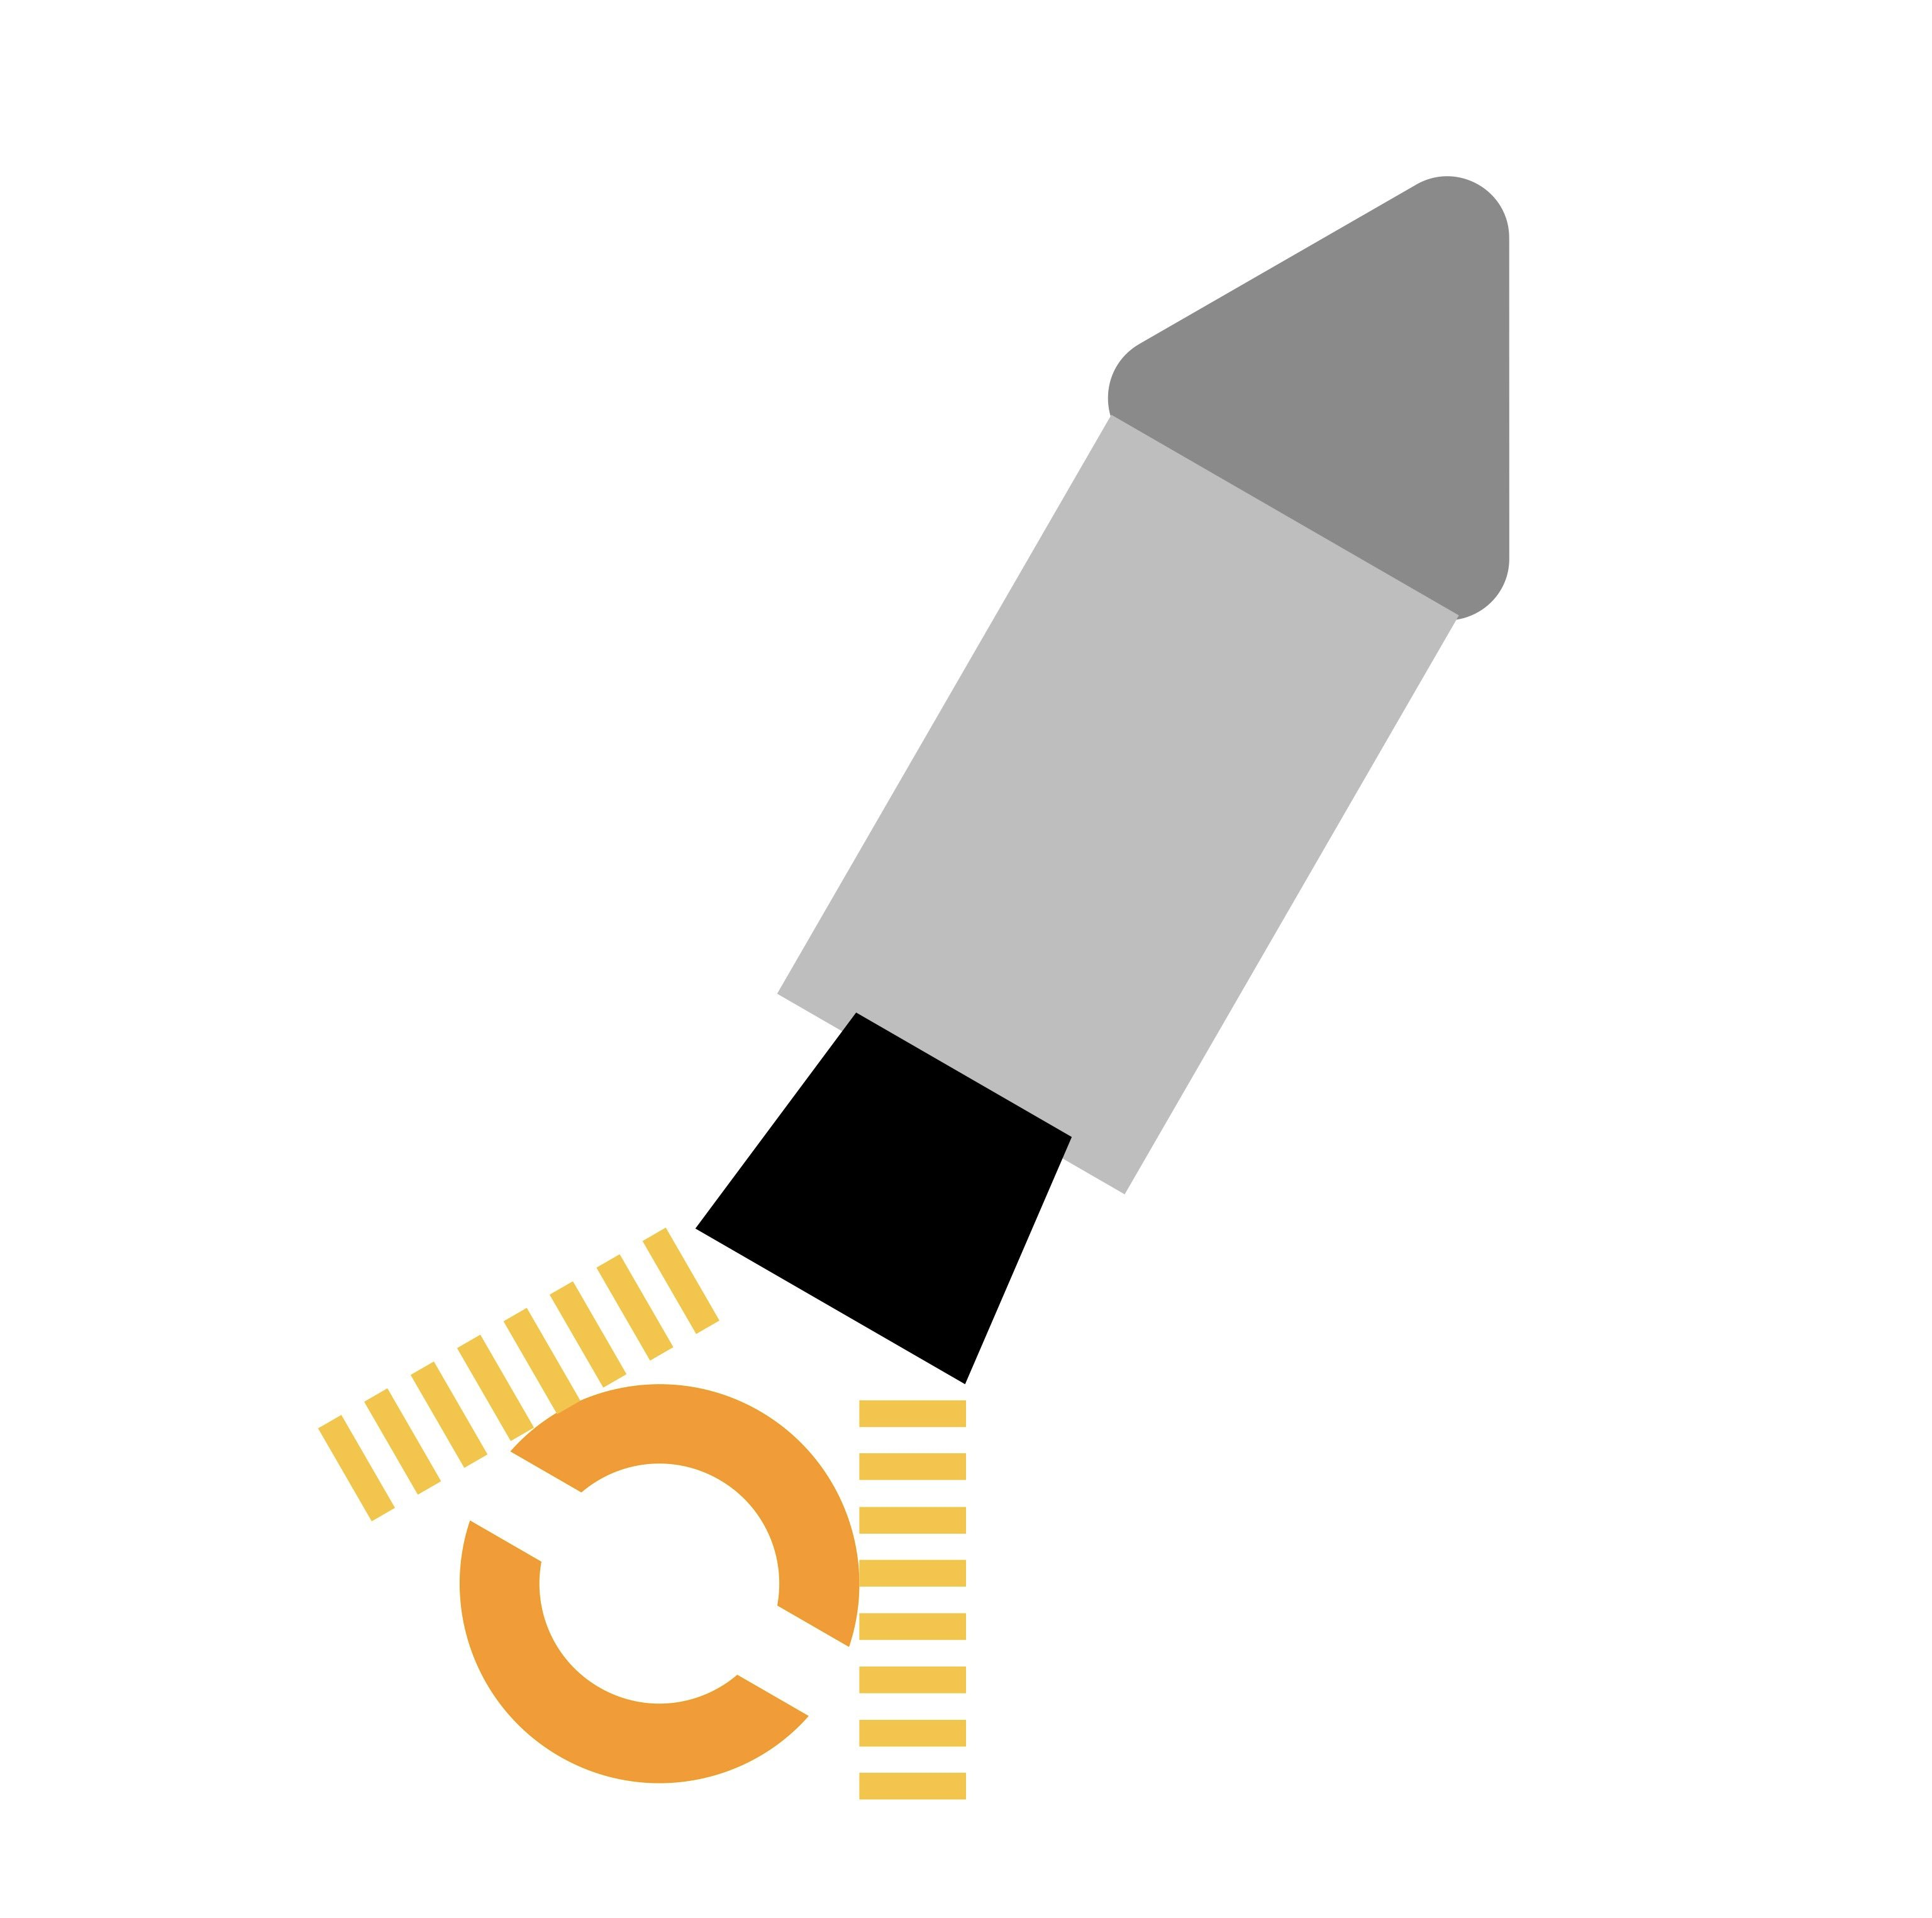
\includegraphics[width=0.15\textwidth]{img/mzpfp1.jpg}
    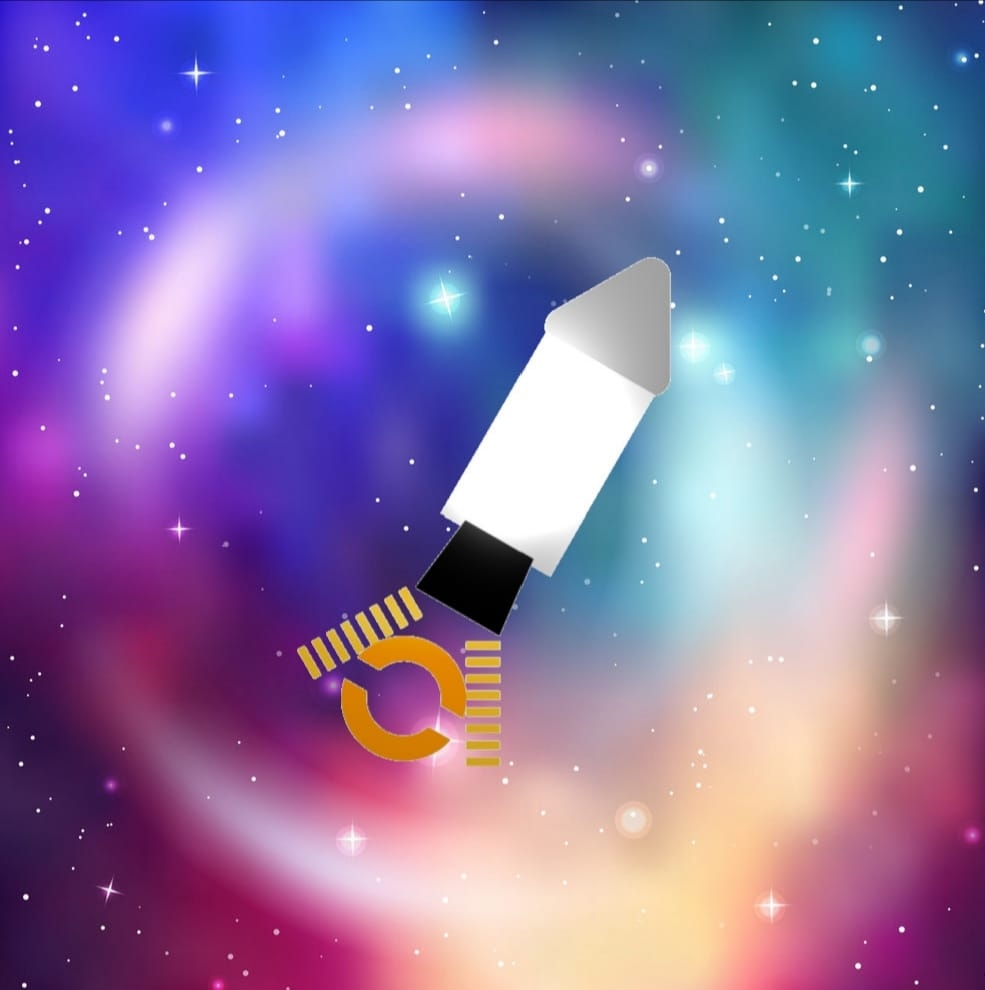
\includegraphics[width=0.15\textwidth]{img/mzpfp2.jpg}
    \par\vspace{1cm}
	{\Large \textsc{Astronomy POSN Summaries (AstroNotes)}\par}
    \vspace{0.25cm}
	{\Large \textsc{ไฟล์สรุปสำหรับ สอวน. ดาราศาสตร์}\par}

	\vspace{2cm}
	{\LARGE\bfseries Introduction to Astronomy\par}
    \vspace{0.25cm}
    {\LARGE\bfseries ปฐมบทสู่ดาราศาสตร์\par}

	\vspace{1cm}
	{\Large\itshape กิตติพัศ พงศ์อรุโณทัย\par}
    \vspace{0.25cm}
    {\large\itshape โรงเรียนกำเนิดวิทย์\par}
    {\itshape ศูนย์ สอวน. ดาราศาสตร์ โรงเรียนมหิดลวิทยานุสรณ์ และโรงเรียนสวนกุหลาบวิทยาลัย}
	\vfill
% Bottom of the page
	{\large \today\par}
\end{titlepage}

\section{ดาราศาสตร์คืออะไร}
ดาราศาสตร์ คือวิชาที่ศึกษาท้องฟ้าและวัตถุต่างๆ เช่นดาวฤกษ์ ดาวเคราะห์ เนบิวลา กระจุกดาว กาแล็กซี่ และอีกมากมาย โดยวิธีที่เราใช้ศึกษา คือการนำฟิสิกส์และคณิตศาสตร์มาประยุกต์ใช้ (ถ้าคุณคิดว่าดาราศาสตร์คือวิชาดูดาว ก็ขอแสดงความเสียใจด้วยนะครับ สิ่งนั้นจะได้ทำเพียงประมาณ 10\% ของเวลาทั้งหมด) แม้ว่าวิชาดาราศาสตร์จริงๆ แล้วกว้างมาก ใน AstroNotes เราจะเน้นเนื้อหาที่เป็นประโยชน์ต่อสอวน. เท่านั้น

\section{ส่วนประกอบของดาราศาสตร์}
ในการเรียนรู้ของค่ายสอวน. เรามักจะแบ่งดาราศาสตร์เป็น 4 ส่วนดังนี้
\begin{enumerate}
    \item ทรงกลมท้องฟ้า (Celestial Sphere)
    \item กลศาสตร์ท้องฟ้า (Celestial Mechanics)
    \item การแผ่รังสีของวัตถุดำ (Blackbody Radiation)
    \item ฟิสิกส์ดาราศาสตร์ (Astrophysics)
\end{enumerate}
ศูนย์ต่างๆ จะมีการแบ่งที่แตกต่างกันไป บางเรื่องที่อาจนับว่าเป็นส่วนย่อย ดังนั้นใน AstroNotes จะเป็นการแบ่งที่ย่อยที่สุด เช่น เอกภพวิทยา (Cosmology) จะกลายเป็นส่วนหนึ่ง \\
นอกจากนี้ เรามักจะต้องอาศัยความรู้หลายอย่าง ตัวอย่างที่เห็นชัดมาก คือเรื่องของดาวคู่ (Binary Star) ที่อาศัยความรู้ทุกด้าน ดังนั้นเนื้อหาเหล่านี้ จะอยู่ใน "Applied Astronomy"

\section{วัตถุท้องฟ้า}
ในทางดาราศาสตร์ จะมีวัตถุอยู่หลายชนิดที่ควรรู้จัก ซึ่งเราจะพูดถึงกัน
\end{document}
